\section{Robustness to Static Parameter Deviations \label{sec:static}}
We have formulated the QOC
problem as an open-loop optimization problem, i.e.
we do not incorporate feedback from the experiment in optimization.
However, the device typically deviates from the Hamiltonian we use in optimization,
leading to poor experimental performance. We combat errors
of this form using robust control techniques,
making the state evolution insensitive
to Hamiltonian parameter deviations. As an example,
we mitigate errors arising from the drift and finite measurement
precision of the qubit frequency which modifies \eqref{eq:hamiltonian}
by $f_{q} \gets f_{q} + \delta f_{q}$.
We consider three robust control techniques:
the sampling method, the unscented sampling method,
and the derivative method.

The sampling method simultaneously optimizes over copies of a state,
each of which evolves with a distinct deviant parameter value.
We append four sets of two sample states $\psi^{\pm}$
to the augmented state vector \eqref{eq:astatecontrols}.
We initialize each pair of samples in the same state.
The four initial states are chosen so that their outerproducts
span the operators on the Hilbert space
$\{\ket{0}, \ket{1}, (\ket{0} + i\ket{1}) / \sqrt{2},
(\ket{0} - \ket{1}) / \sqrt{2}\}$ \cite{chow2009randomized}.
The discrete dynamics \eqref{eq:dyn_con} is modified so that the
samples evolve under the Hamiltonian given in \eqref{eq:hamiltonian}
with $f_{q} \gets f_{q} \pm \sigma_{f_{q}}$ for a fixed $\sigma_{f_{q}}$.
The final state
for each sample is the image of its initial state
under the desired gate. The infidelity between
the samples and their final states are penalized
by adding a term
$\sum_{k=1}^{N} q_{k} (1 - {\lvert \braket{\psi^{\pm}_{k}}{\psi_{f}} \rvert}^{2})$
to the objective \eqref{eq:costfun}.

For the unscented sampling method, we append $2(2n + d)$ samples
to the augmented state vector \eqref{eq:astatecontrols}
for each initial state in the operator basis. Here $2n = 4$ is twice the
dimension of the Hilbert space, resulting from the isomorphism \eqref{eq:isomorphism},
and $d = 1$ is the number of deviant parameters. The samples
represent a Gaussian distribution over the $2n$
elements of the initial state, modeling
the uncertainty in the state as a result of the uncertainty in
the deviant parameter. Each sample evolves under the Hamiltonian
given in \eqref{eq:hamiltonian} with $f_{q} \gets f_{q} + \delta f_{q}$.
We determine the qubit frequency detuning $\delta f_{q}$
at each knot point using the statistics of the samples.
We modify the discrete dynamics \eqref{eq:dyn_con} to
evolve the samples under the deviant Hamiltonian
and then apply the unscented transformation to the ensemble
of samples,
accurately preserving the first and second moments
of the distribution.
We penalize the infidelity between the samples and their final states
by adding an infidelity contribution to \eqref{eq:costfun}
as in the sampling method.
A detailed procedure for the unscented transformation is given
in Appendix \ref{appendix:unscented}.

The derivative method penalizes the sensitivty of the state
to the deviant parameter, which is encoded in the ($l$\textsuperscript{th}-order)
derivative $\partial_{f_{q}}^{l} \psi$. In the $m$\textsuperscript{th}-order
derivative method, we append all state derivatives of order $1, \dots, m$
to the augmented state vector \eqref{eq:astatecontrols}
for each initial state in the operator basis.
We penalize the norms of the state derivatives
in \eqref{eq:costfun} by setting the corresponding final states to zero.
We could obtain the state derivatives in the discrete dynamics \eqref{eq:dyn_con}
with backwards mode differentiation.
Naive automatic differentiation 
would differentiate all dynamics at knot points
$1, \dots, k - 1$ to obtain the state derivative at knot point $k$, requiring
$O(N^{2})$ matrix multiplications. Instead, we 
employ forwards mode differentiation on the TDSE to obtain coupled dynamics
which require $O(N)$ matrix multiplications to integrate.
For example, the dynamics for the $1$\textsuperscript{st}-order derivative method are:
\begin{align}
  i \hbar \frac{d}{dt} \ket{\psi} &= H \ket{\psi}\\
  i \hbar \frac{d}{dt} \ket{\partial_{f_{q}}\psi} &=
  H \ket{\partial_{f_{q}} \psi} +
  (\partial_{f_{q}} H) \ket{\psi}
  \label{eq:d1dyn}
\end{align}
Exponential integrators that account for the non-linear
term in \eqref{eq:d1dyn} are used to efficiently integrate the coupled dynamics,
see Appendix \ref{appendix:derivative}. For runtimes
and complexity analyses for the three robust control methods,
consult Appendix \ref{appendix:time}.

We challenge these methods to achieve
a $Z/2$ gate subject to a static qubit frequency detuning.
We take $\sigma_{f_{q}} / f_{q} = 1\%$ to be one standard devation, and equip
the sampling methods accordingly. We compute gate errors for each method
by evolving the system under the Hamiltonian in \eqref{eq:hamiltonian}
with the optimized flux amplitude and $f_{q} \gets f_{q} + \delta f_{q}$
at the stated qubit frequency detuning.

We compare the numerical methods
to an analytically derived $Z/2$ gate, see Figure \ref{fig:statica}. 
The analytic gate corresponds to
idling at the flux frustration point $a = 0$. It
is at the device's speed limit for a $Z/2$ gate $t_{Z/2} = 1 / 4 f_{q}$ and
is simple to derive. Its erroneous rotation angle
$2 \pi t_{Z/2} \delta f_{q}$ is linearly sensitive to
the qubit frequency detuning, resulting in a gate error that is quadratically sensitive
to the qubit frequency detuning.
At a one-percent
qubit frequency detuning ($\delta f_{q} / f_{q} = 1\%$)
the analytic gate achieves a gate error $\sim 4.5 \cdot 10^{-5}$,
which is sufficient for quantum error correction.
Although the analytic $Z/2$ gate performs well, it
only works at the gate time $t_{Z/2}$. The ability to perform $Z$
rotations in arbitrary times is critical
for multi-qubit experiments, where the qubits operate at different
frequencies $f_{q, i} \neq f_{q, j}$.
Each numerical method can find solutions at
all gate times above $t_{Z/2}$, see Figure \ref{fig:staticb}.
These numerical methods offer an effective scheme for synchronizing
multi-qubit experiments.

The sampling and unscented sampling methods combine idling periods
with time-anti-symmetric ramps.
The gate error at $\delta f_{q} / f_{q} = 1\%$ for the sampling method
does not improve substantially over the
range of gate times. The unscented sampling method
achieves linear decreases in its gate error at
$\delta f_{q} / f_{q} = 1\%$ with longer gate times
until half the Larmor period $1 / 2 f_{q}$ after which it achieves a consistent
gate error $\sim 3.5 \cdot 10^{-5}$.

The derivative methods converge on qualitatively similar solutions that
use fast triangle pulses at the boundaries and balance time
on either side of the flux-frustration point symmetrically at low amplitudes.
Both methods achieve a super-linear scaling in their gate error as
a function of their gate time.
We believe the 1\textsuperscript{st}-order method outperforms the 2\textsuperscript{nd}-order
method due to the low contribution of second-order
terms to the gate error in this deviation regime, see Appendix \ref{appendix:derivative}.
The gate error for the 1\textsuperscript{st}-order
derivative method approaches zero at the Larmor period $1 / f_{q}$, see Figure \ref{fig:staticc}.
This result mimics the
ability of composite pulses to mitigate parameter deviation errors to arbitrary
order with sufficiently many pulses \cite{merrill2014progress}.
It is difficult to choose an appropriate composite pulse
for the problem studied here due to our Hamiltonian and experimental constraints.
We propose comparisons between composite pulses and numerical techniques
for future work.

%% F3
\begin{figure*}[ht]
  \begin{subfigure}{.4\textwidth}
    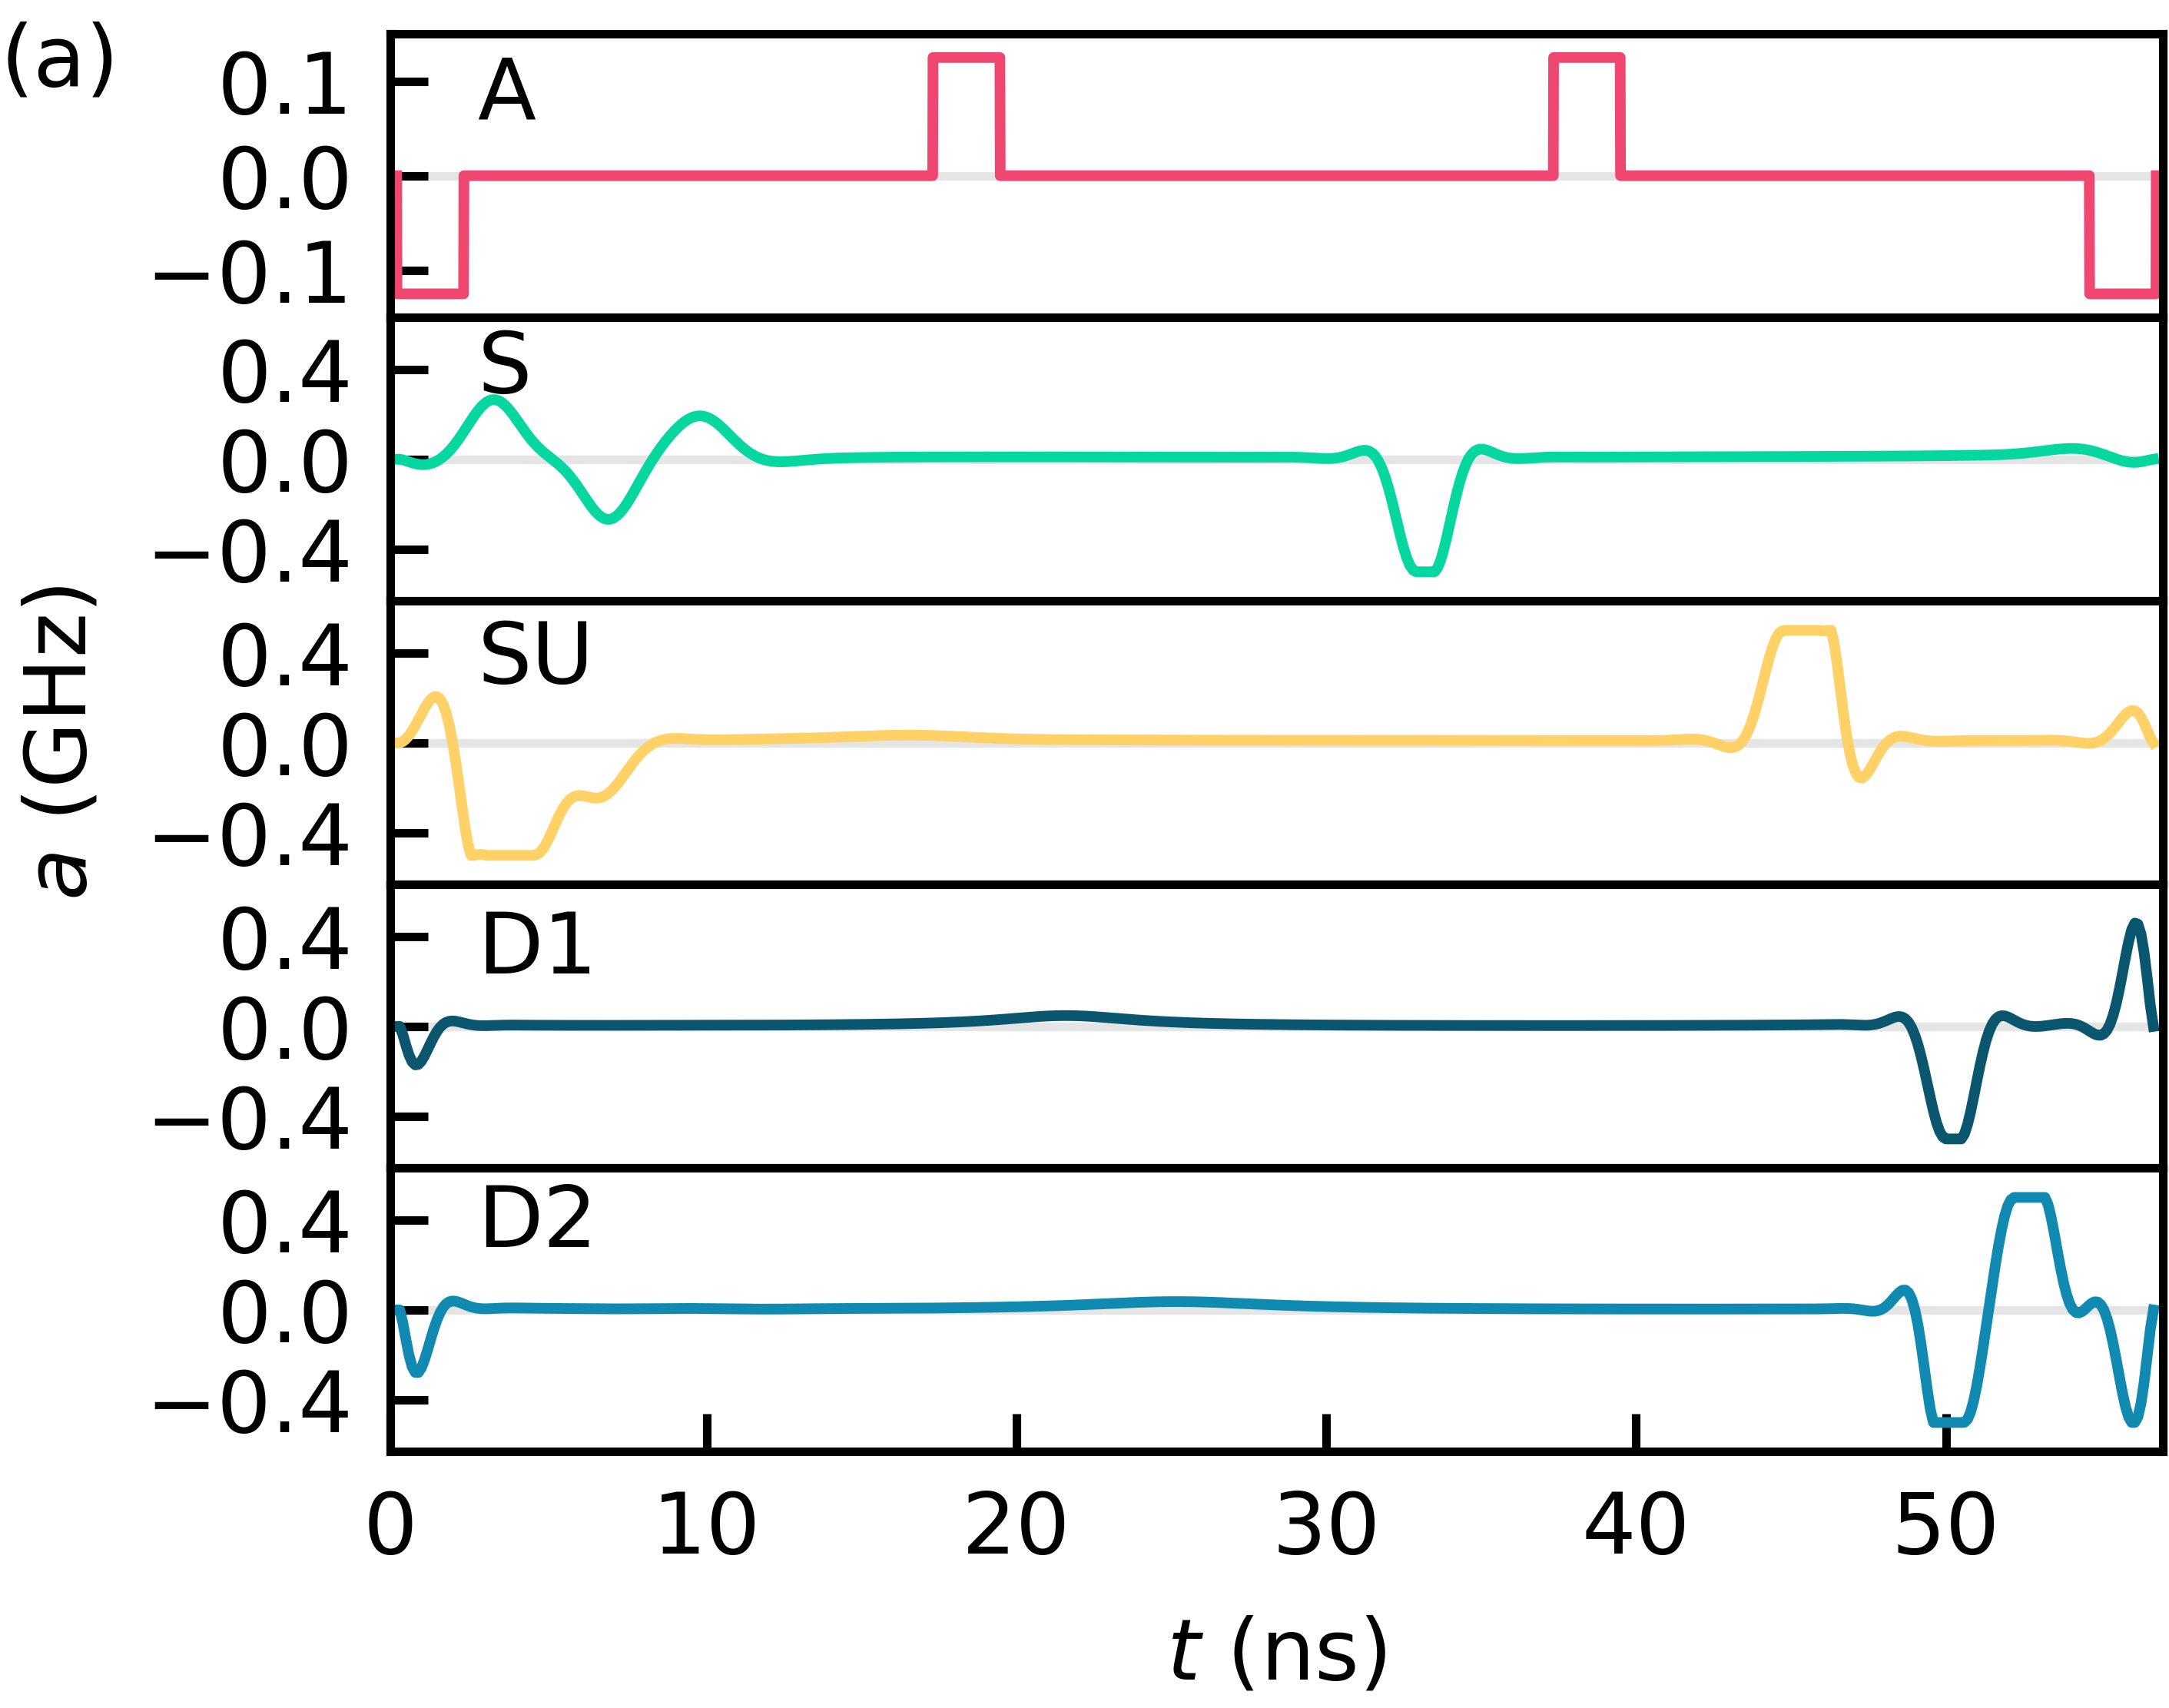
\includegraphics[width=\linewidth]{assets/f3a.png}
    \caption{}
    \label{fig:stochastica}
  \end{subfigure}\hspace{0.05\textwidth}
  \begin{subfigure}{.4\textwidth}
    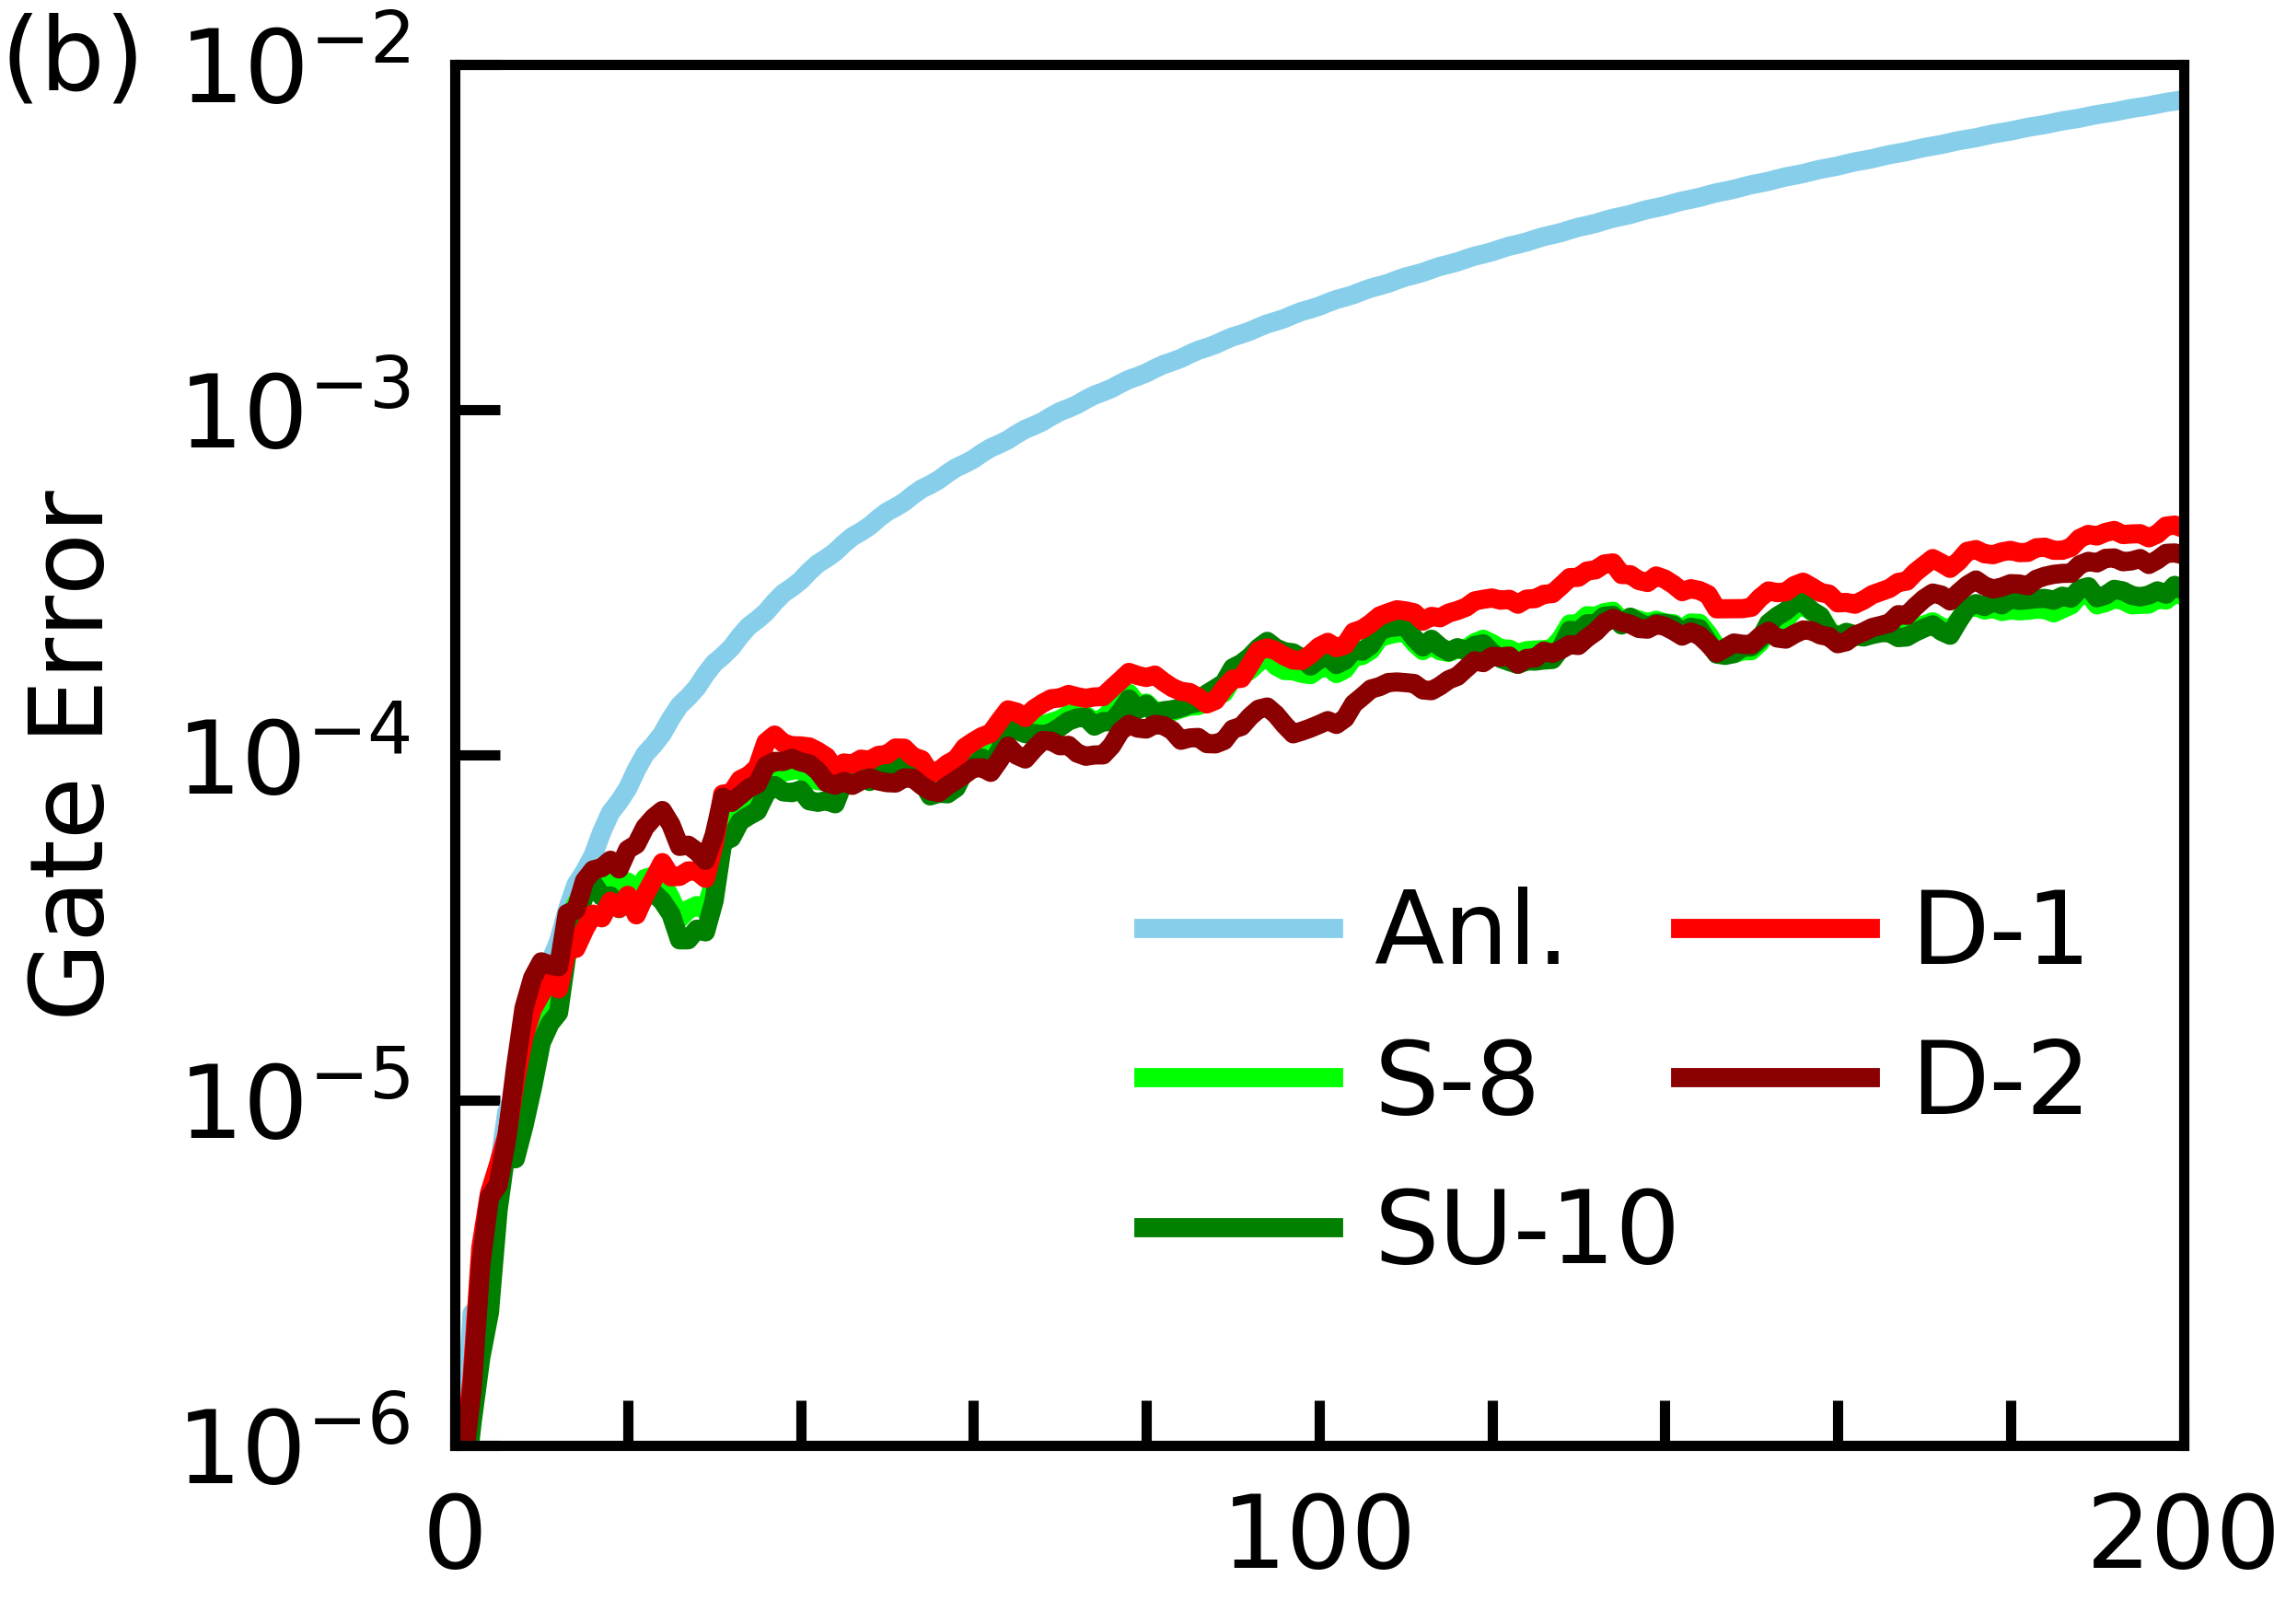
\includegraphics[width=\linewidth]{assets/f3b.png}
        \caption{}
    \label{fig:stochasticb}
  \end{subfigure}
  \caption{
    (a) $X/2$ gates robust to flux amplitude offsets constructed with the analytic,
    sampling, unscented sampling, and the 1\textsuperscript{st}-
    and 2\textsuperscript{nd}-order derivative methods. The gates shown
    are the solutions at the analytic gate time.
    (b) Simulation of stochastic 1/$f$ flux noise for
    successive gate applications. The cumulative
    gate error is computed after each gate application.
  }
  \label{fig:stochastic}
\end{figure*}
